% !TEX root = isae-beamer-template.tex

% Recall the outline at each section
\begin{frame}
  \frametitle{Serielle Kommunikation über UART}
	    \begin{column}{1\linewidth}
	    	Übersicht über die Hardware-Anbindung UART:\\
	    	Achtung: Robo V1 über \textbf{Segger RTT}
	    	\begin{center}
	    		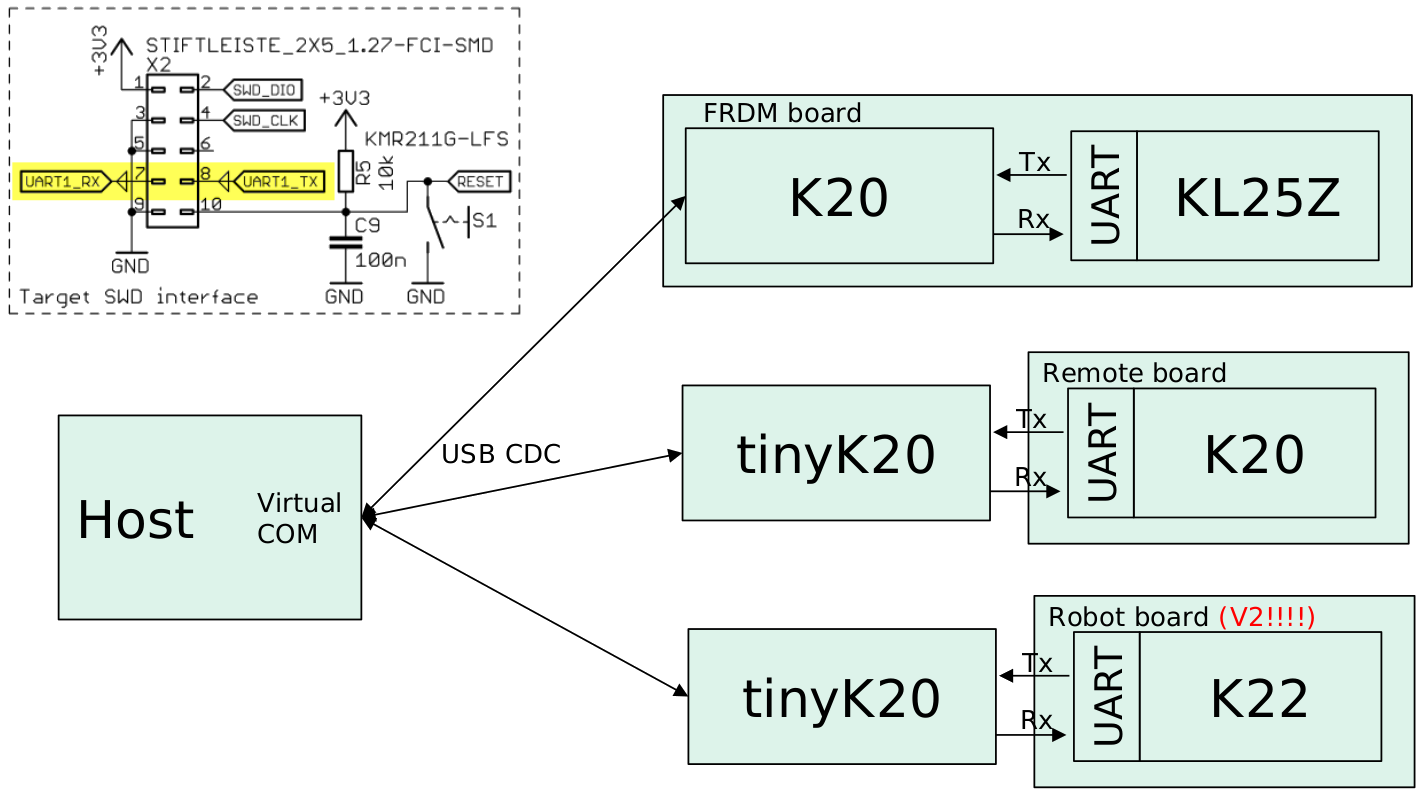
\includegraphics[width=0.8\textwidth]{images/UART_HW_Mapping.png}
	    	\end{center}
	    \end{column}
\end{frame}

\begin{frame}
  \frametitle{Processor Expert Komponenten}
  	\begin{columns}
	    \begin{column}{0.45\linewidth}
	    	\begin{itemize}
	    	\item CLS1:Shell in Processor Expert
	    	\item Blockierendes Senden einschalten
	    	\item WAIT1 verwenden
	    	\item Timeout: Wartezeit zwischen dem Senden. \\0 = blockierend
	    	\item Wait Time: Wenn der Puffer voll ist, wie lange soll gewartet werden?
	    	\item Console Interface: AS1
	    	\end{itemize}
	    \end{column}
	    \begin{column}{0.45\linewidth}
	    	\begin{center}
	    		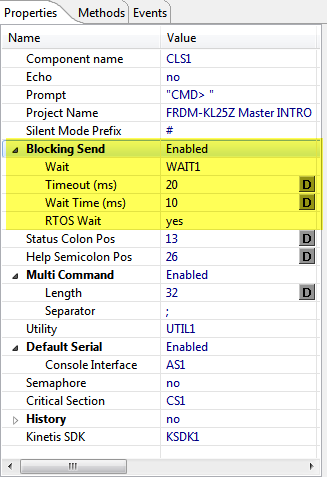
\includegraphics[width=0.8\textwidth]{images/CLS1_shell.png}
	    	\end{center}
	    \end{column}
	\end{columns}
\end{frame}

\begin{frame}
  \frametitle{AS1 Einstellungen}
  	\begin{columns}
	    \begin{column}{0.45\linewidth}
	    	\begin{itemize}
	    	\item Channel: UART0
	    	\item Input buffer size: 32Bit empfohlen
	    	\item Output buffer size: 32Bit empfohlen
	    	\item Receiver: UART0\_RX
	    	\item Transmitter: UART0\_TX
	    	\item Baudrate setzen und mit Terminal abgleichen
	    	\end{itemize}
	    \end{column}
	    \begin{column}{0.45\linewidth}
	    	\begin{center}
	    		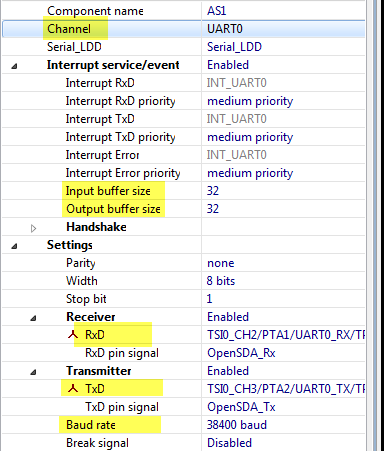
\includegraphics[width=1\textwidth]{images/CLS1_shell_2.png}
	    	\end{center}
	    \end{column}
	\end{columns}
\end{frame}

\begin{frame}[fragile]
  \frametitle{Anschluss am PC/ Notebook}
	    \begin{column}{1\linewidth}
	    	\textbf{Port finden bei Windows:}\\
	    	\begin{center}
	    		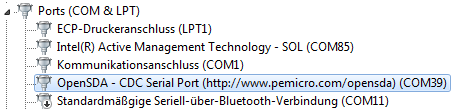
\includegraphics[width=0.7\textwidth]{images/COM_Windows.png}
	    	\end{center}
	    	Achtung: Bei Windows 7 kann es passieren, dass der Port blockiert!\\[0.2cm]
	    	\textbf{Bei Linux:}\\
	    	Terminal öffnen und den untenstehenden Befehl ausführen.
			\begin{verbatim}
				dmesg | grep tty
			\end{verbatim}
			\begin{center}	    	
	    		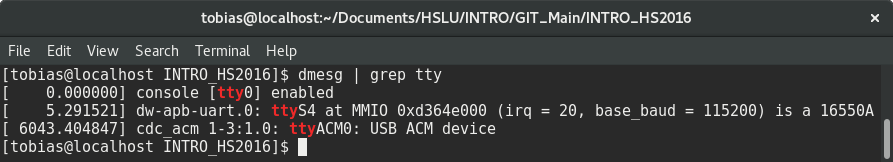
\includegraphics[width=0.7\textwidth]{images/Console_Result_dmesc.png}
	    	\end{center}
	    \end{column}
\end{frame}

\begin{frame}
  \frametitle{Shell Standard I/O}
	    \begin{column}{1\linewidth}
	    	\textbf{I/O Strukturen mit Callback}\\
			\begin{itemize}
			\item \textbf{Stdin}: Zeichen (char) lesen
			\item \textbf{Stdout}: Zeichen schreiben
			\item \textbf{Stderr}: Zeichen schreiben
			\item \textbf{KeyPressed}: Zeichen anstehend in Stdin?
			\end{itemize}
	    	\textbf{Zeichenketten (Strings) und Zahlen senden (nicht printf):}
			\begin{center}	    	
	    		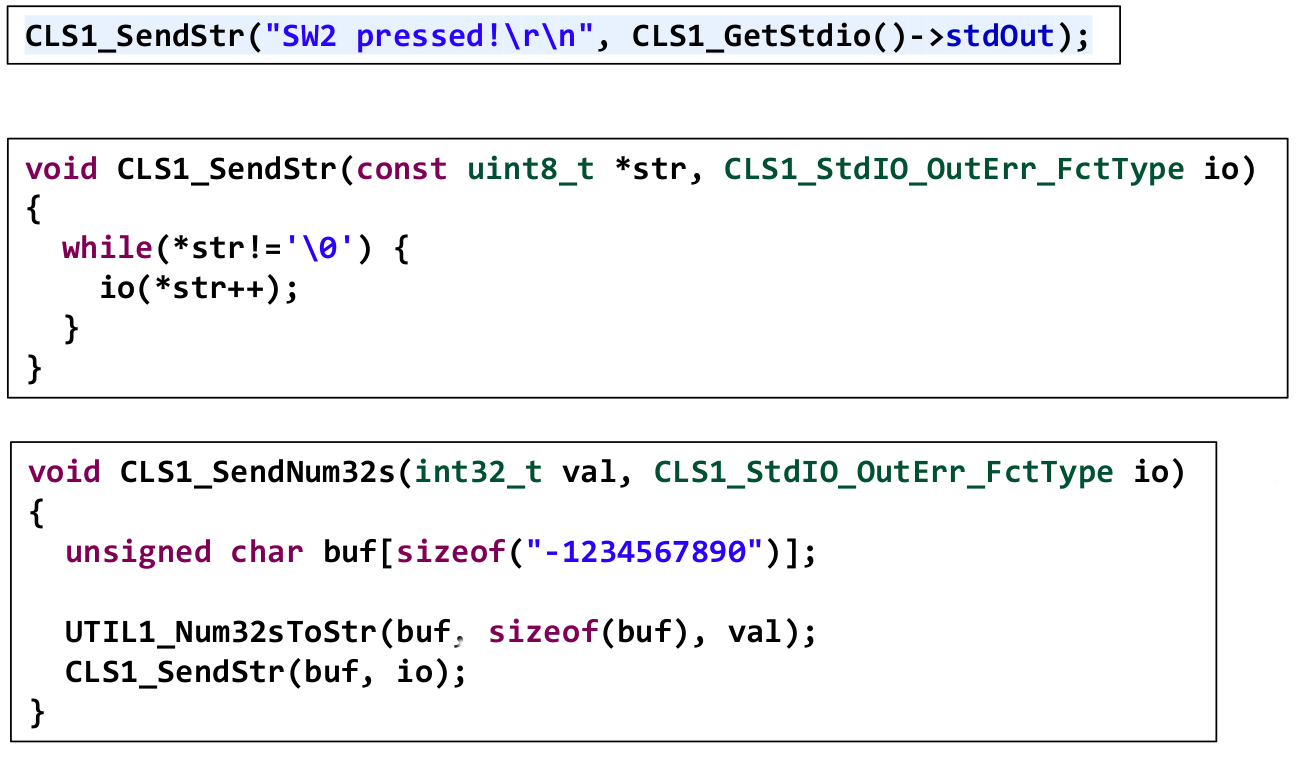
\includegraphics[width=0.6\textwidth]{images/Write_chars.png}
	    	\end{center}	    	
	    \end{column}
\end{frame}